\subsection{Блочно-структурированная расчетная сетка \\ и организация межпроцессных обменов}

Одним из наиболее распространенных типов расчетных сеток, используемых для численных расчетов, является блочно-структурированная сетка\label{term:mesh_block_struct2}, состоящая из нескольких блоков, некоторые из которых имеют общие границы.
Такая структура позволяет выполнять вычисления для различных блоков независимо друг от друга, обмениваясь общими данными на границах по мере необходимости.
Для эффективного проведения вычислений на блочно-структурированных сетках с использованием суперкомпьютера важную роль имеет реализация расчетной сетки в виде внутреннего представления и организация механизма межпроцессного обмена данными между соседними блоками сетки \cite{Rybakov2017Mesh}.

\subsubsection{Cтруктура блочно-структурированной сетки}

Будем рассматривать блочно-структурированные сетки, состоящие из отдельных блоков, каждый из которых представляет собой упорядоченный трехмерный массив ячеек, имеющих форму кубоида.
Упорядоченность размещения ячеек обеспечивает быстрый доступ к ячейками по индексам и снижает требования к объему памяти, однако строить блочно-структурированные сетки гораздо сложнее, чем неструктурированные.

Блоки блочно-структурированной сетки могут иметь сложную форму.
Для доступа к отдельным ячейкам блока вводятся три индекса, связанные с криволинейной системой координат блока.
Система координат задается тремя линиями координат $(I, J, K)$, каждая из которых связывает пары противоположных граней блока.
Для наглядности будем изображать блоки сетки в виде прямоугольных параллелепипедов, как показано на рис.~\ref{fig:text_2_block_block} слева.

\begin{figure}[ht]
\centering
\begin{tabular}{ll}
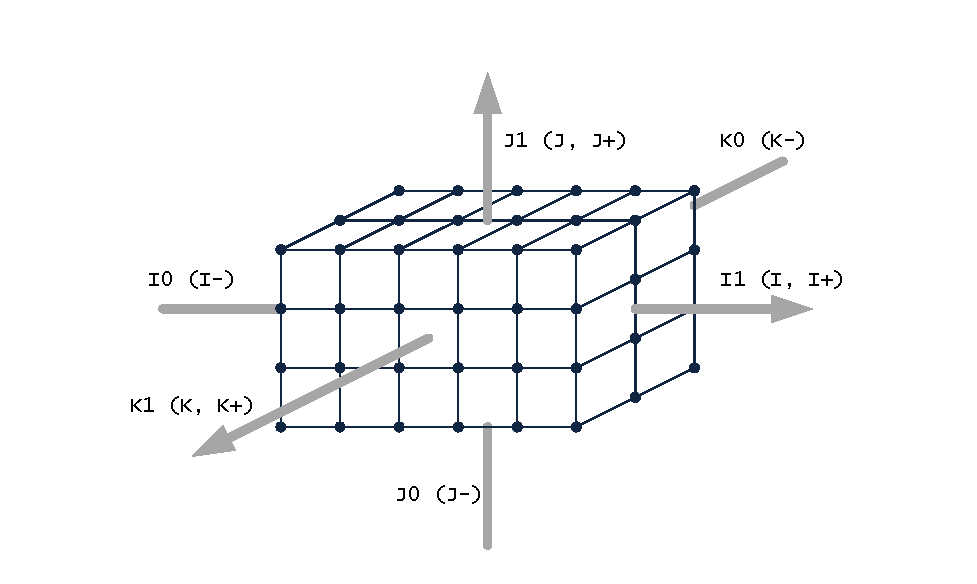
\includegraphics[width=0.45\textwidth]{./pics/text_2_block/1-block.pdf}
&
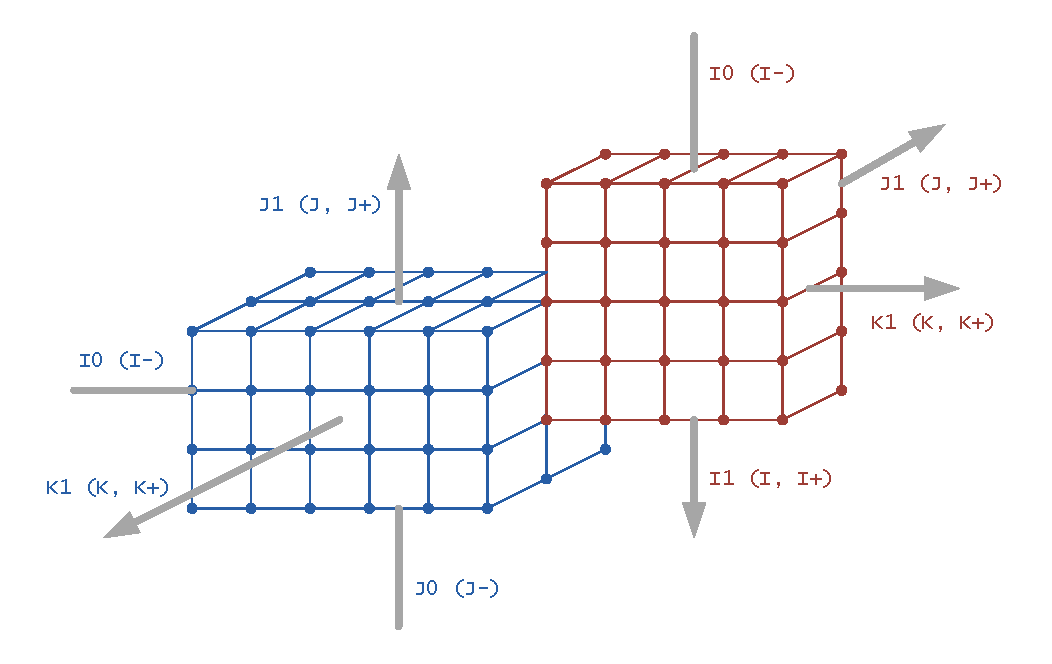
\includegraphics[width=0.45\textwidth]{./pics/text_2_block/2-block-block.pdf}
\end{tabular}
\singlespacing
\captionstyle{center}\caption{Блок сетки (слева) и касание блоков (справа).}
\label{fig:text_2_block_block}
\end{figure}

Блоки могут граничить между собой.

\begin{definition}
Интерфесом\label{term:block_interface} будем называть описание области границы одного блока, по которой он касается другого блока расчетной сетки.
\end{definition}

Один интерфейс описывает соприкосновение двух блоков прямоугольными подобластями своих граней.
При этом системы координат двух соседних блоков не обязаны согласовываться между собой.
Пример касания двух блоков приведен на рис.~\ref{fig:text_2_block_block} справа.

Выполнение расчетов на сетке носит итерационный по времени характер.
Для каждой итерации по времени выполняется пересчет данных ячеек согласно той или иной вычислительной схеме.
Во время обработки одной ячейки возникает потребность обращаться за данными к другим ячейкам (например, для выполнения аппроксимации частных производных каких-либо величин), находящимся рядом с рассматриваемой (в простейшем случае это просто соседние по граням ячейки, но могут использоваться и используются более сложные структуры).

\begin{definition}
Совокупность ячеек расчетной сетки, данные которых используются при обработке конкретной ячейки, называют вычислительным шаблоном, или вычислительной молекулой, или вычислительной окрестностью этой ячейки\label{term:cell_calc_template}.
\end{definition}

На рис.~\ref{fig:text_2_block_cell_delta} показаны примеры вычислительных окрестностей ячейки.

\begin{figure}[ht]
\centering
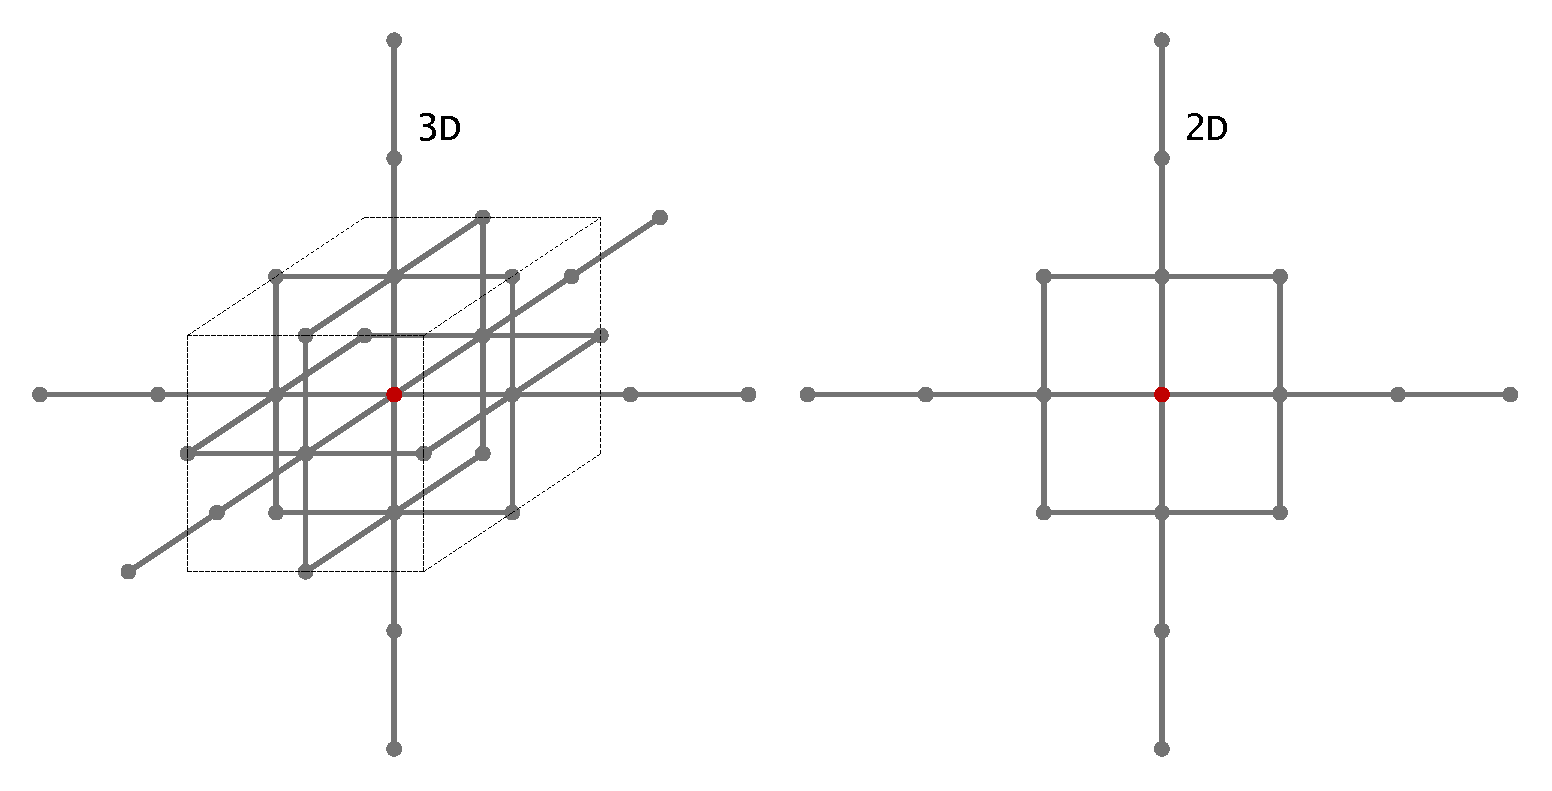
\includegraphics[width=0.8\textwidth]{./pics/text_2_block/3-cell-delta.pdf}
\singlespacing
\captionstyle{center}\caption{Примеры вычислительных окрестностей ячеек сетки.}
\label{fig:text_2_block_cell_delta}
\end{figure}

В дальнейшем для большей наглядности будем изображать блоки в двумерном виде (с системой координат $IJ$).

Во время произведения расчетов различные блоки сетки обрабатываются независимо друг от друга.
При этом для некоторых ячеек обрабатываемого блока их вычислительные окрестности выходят за границу блока и затрагивают соседние блоки.
Для эффективного счета необходимо обеспечить функционал быстрого обмена данными между блоками.
Если два соседних блока обрабатываются на разных узлах суперкомпьютерного кластера, то для обмена данными между ними нужно использовать MPI обмены.
Приведем классификацию ячеек внутри блока сетки (см. рис.~\ref{fig:text_2_block_block_cells}) слева.

\begin{figure}[ht]
\centering
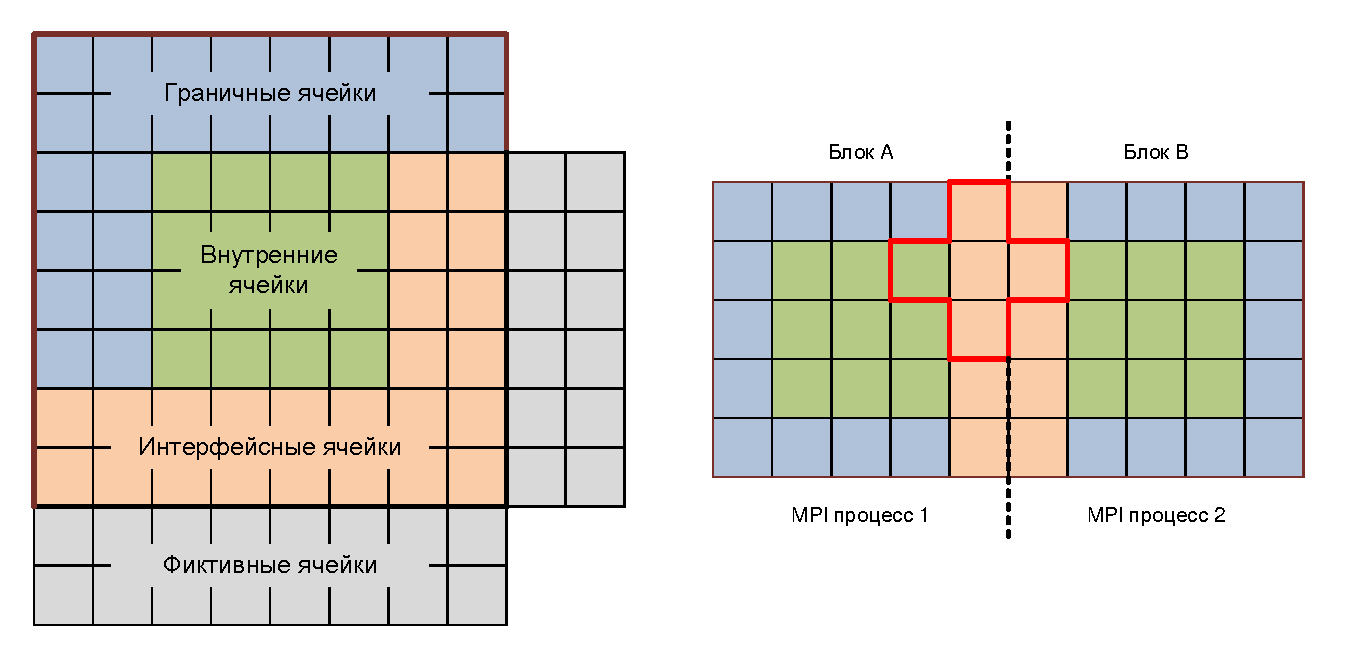
\includegraphics[width=0.8\textwidth]{./pics/text_2_block/4-block-cells.pdf}
\singlespacing
\captionstyle{center}\caption{Ячейки разных типов.}
\label{fig:text_2_block_block_cells}
\end{figure}

\begin{definition}
Внутренними ячейками\label{term:cell_block_inner} (Inner Cells) будем называть те ячейки блока, вся окрестность которых лежит внутри того же блока.
\end{definition}

\begin{definition}
Ячейки, не являющиеся внутренними ячейками блока, будем называть граничными ячейками\label{term:cell_block_border} (Border Cells).
\end{definition}

\begin{definition}
Если окрестность ячейки частично накрывает один из соседних блоков, то такую ячейку будем относить к интерфейсным ячейкам\label{term:cell_block_interface} (Interface Cells), так как ее окрестность пересекает интерфейс блока.
\end{definition}

\begin{definition}
Если окрестность ячейки частично накрывает некоторый блок, который обрабатывается в другом узле суперкомпьютера, то будем относить ее к ячейкам MPI обмена (MPI Cells)\label{term:cell_block_mpi}, так как для получения данных этой окрестности нужно использовать средства межпроцессного обмена (см. рис.~\ref{fig:text_2_block_block_cells} справа).
\end{definition}

При обработке ячеек MPI обмена мы должны обращаться за данными к другому процессу.
Если делать это только по мере необходимости, то придется совершать большое количество обменов, что негативно скажется на производительности.
Поэтому для повышения быстродействия вместо этого для блока заводится специальный слой внешних ячеек, куда копируются все необходимые данные из соседних процессов, которые могут понадобиться при обработке блока.
Такие ячейки будем называть фиктивными\label{term:cell_block_ghost}.

\begin{definition}
Фиктивными ячейками блока будем называть дополнительно созданные для этого блока ячейки, которые содержат скопированные из соседних блоков данные, необходимые для выполнения вычислений в рассматриваемом блоке.
Множество фиктивных ячеек блока также будем называть его теневым слоем\label{term:block_shadow_layer}.
\end{definition}

Ширина теневого слоя блока определяется размером вычислительного шаблона обработки ячейки.
Фиктивные ячейки могут не являться ячейками в физическом смысле, так как для проведения вычислений необходимы не все данные фиктивных ячеек, но на логическом уровне будем изображать их отдельными ячейками.
Таким образом, объединение всех ячеек блока с множеством фиктивных ячеек является замкнутой структурой, которая более не требует для своей обработки обращений к другим MPI процессам (на одной итерации выполнения расчетов).

Далее опишем основные объекты, используемые для организации работы с блочно-структурированной сеткой, способы описания этих объектов и внутренние структуры, позволяющие эффективно оперировать этими объектами и производить вычисления.

\subsubsection{Основные объекты блочно-структурированной сетки}

В рамках проведения исследований по распараллеливанию вычислений на блочно-структурированных сетках была разработана архитектура расчетной сетки, реализованы ее объекты и инструменты для работы с ней \cite{CertRybakov2020PrepStruct}.

Основным объектом блочно-структурированной расчетной сетки является блок (Block) (см. рис.~\ref{fig:text_2_block_block_and_coords}). 
Блок состоит из трехмерного массива ячеек размера $IS \times JS \times KS$.
Каждая ячейка содержит набор газодинамических параметров, ассоциированных с центром масс ячейки и другие вспомогательные данные.
Также блок содержит данные о всех вершинах своих ячеек, эти данные хранятся в трехмерном массиве размера $(IS + 1) \times (JS + 1) \times (KS + 1)$.

Для определения геометрии блока необходимо задать его линейные размеры и координаты ($X$, $Y$, $Z$) всех его узлов.

\begin{figure}[ht]
\centering
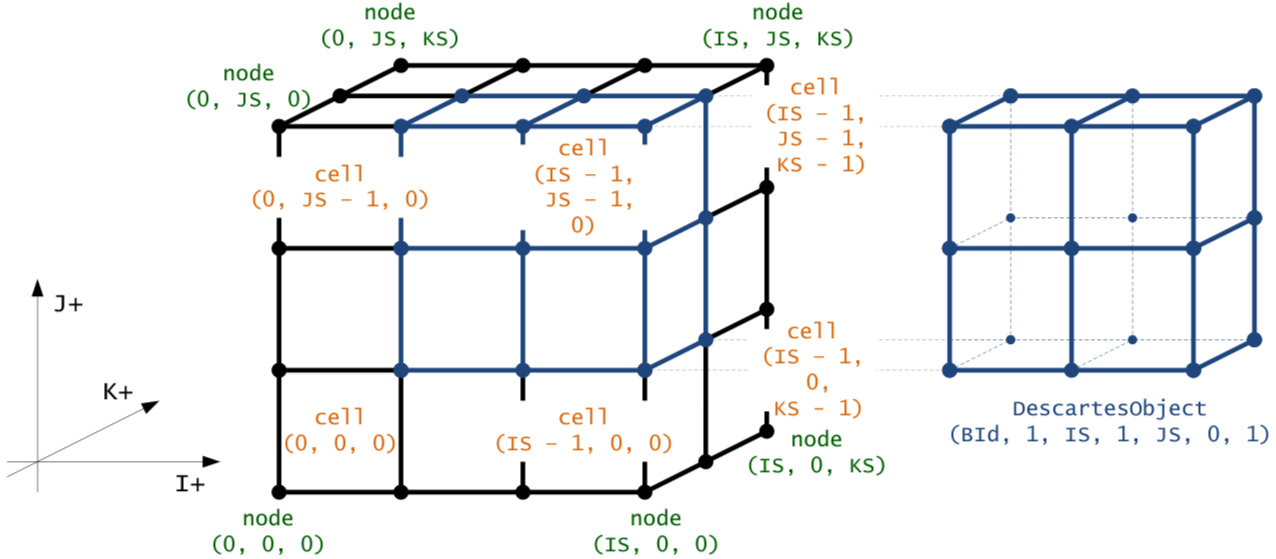
\includegraphics[width=0.7\textwidth]{./pics/text_2_block/6-block-and-coords.png}
\singlespacing
\captionstyle{center}\caption{Блок сетки и координаты его узлов.}
\label{fig:text_2_block_block_and_coords}
\end{figure}

\begin{figure}[ht]
\centering
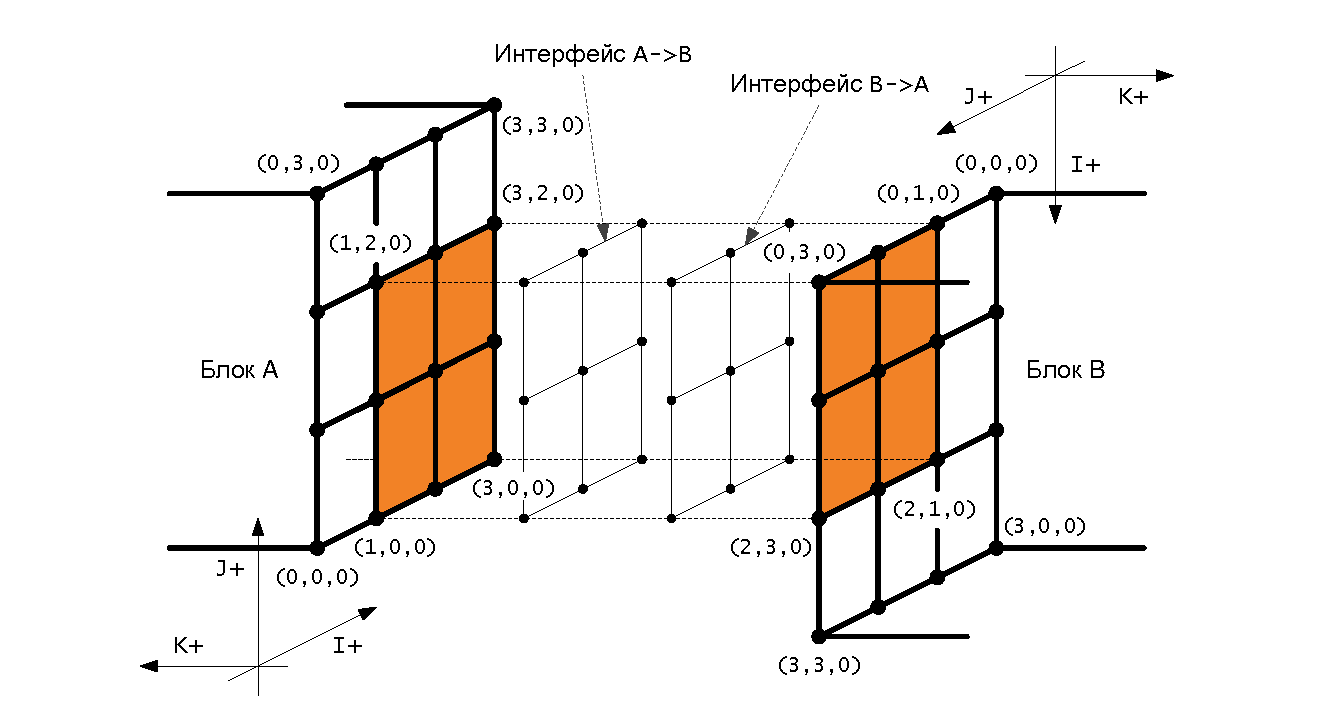
\includegraphics[width=0.8\textwidth]{./pics/text_2_block/7-iface.pdf}
\singlespacing
\captionstyle{center}\caption{Структура интерфейса касания блоков.}
\label{fig:text_2_block_iface}
\end{figure}

Объектом, описывающим соприкосновение двух соседних блоков, является интерфейс (Iface) (см. рис.~\ref{fig:text_2_block_iface}).
Интерфейс является однонаправленным, он сообщает, что у данного блока конкретная прямоугольная
часть границы соприкасается с другим блоком.
Чтобы определить с какой частью другого блока граничит рассматриваемый блок, нужно рассмотреть смежный ему интерфейс.
Таким образом полная информация о касании двух соседних блоков описывается парой смежных интерфейсов.

Интерфейс описывает только касание по ненулевой площади (касание по узлу или ребрам ячеек не рассматривается).
Также возможно обоюдное касание друг друга разных граней одного и того же блока, хотя такие случаи нужно рассматривать отдельно, так как самокасание может потребовать специальной обработки блоков при управлении сеткой.
В общем случае самокасания блоков рекомендуется избегать.

Интерфейс описывается в системе координат того блока, к которому он относится.
Координаты задают размер области соприкосновения по всем трем направлениям.

В приведенном на рис.~\ref{fig:text_2_block_iface} примере два смежным интерфейса, описывающих касание блоков A и B задаются следующим образом: $A(1, 3, 0, 2, 0, 0) \rightarrow B$, $B(0, 2, 1, 3, 0, 0) \rightarrow A$.

\begin{figure}[ht]
\centering
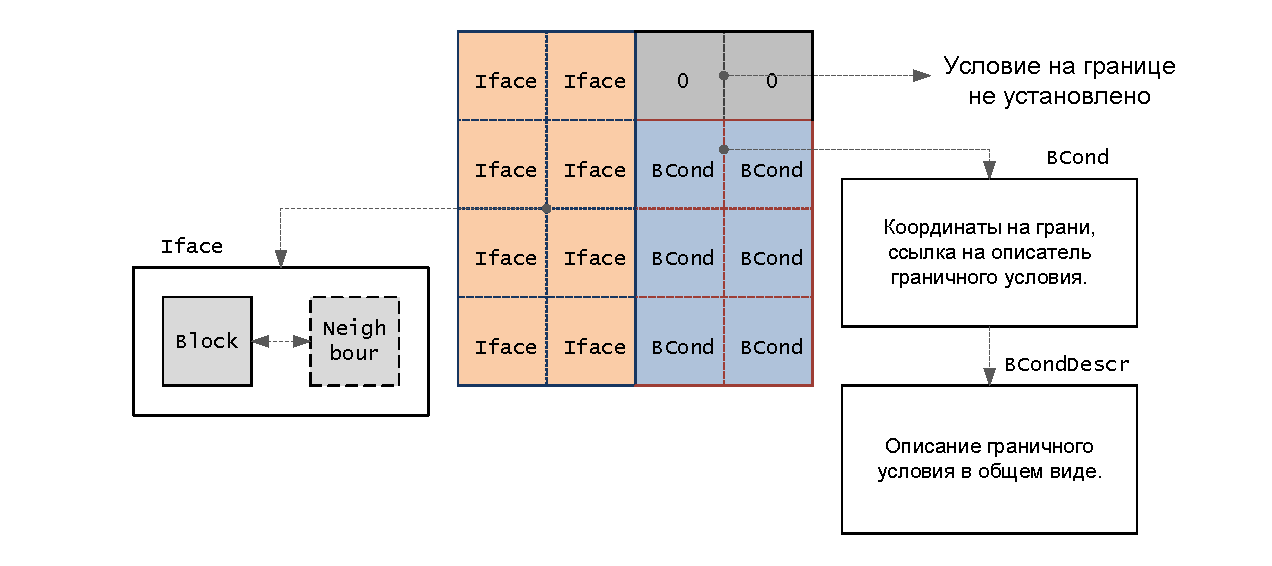
\includegraphics[width=0.8\textwidth]{./pics/text_2_block/8-facet.pdf}
\singlespacing
\captionstyle{center}\caption{Структура грани блока.}
\label{fig:text_2_block_facet}
\end{figure}

То есть для одного интерфейса задается блок, которому этот интерфейс принадлежит, координаты интерфейса в данном блоке и соседний блок.
Этой информации достаточно чтобы полностью определить геометрию касания блоков.
Направление интерфейса можно определить по той координате, протяженность интерфейса по которой равна нулю (в данном случае это координата $K$).
Остается определить только каким образом системы координат двух соседних блоков соотносятся друг с другом.
Это можно сделать, зная координаты узлов соответствующих блоков.

На границе блока кроме другого блока может находиться граница расчетной области.
В этом случае на границе блока необходимо задать граничные условия (BCond).
Граничные условия задаются аналогично интерфейсу (с помощью системы координат блока), однако вместо соседнего блока подается ссылка на описатель граничных условий.
Таким образом и интерфейс и граничное условие являются частным случаем границы блока (Border).

В процессе вычислений необходимо иметь возможность быстро узнать для конкретной граничной ячейки, какого типа граница ей соответствует и быстро найти соответствующий интерфейс или граничное условие.
Для этой цели служат грани блока (Facet)\label{term:block_facet}.
Каждый блок имеет 6 граней (для каждого из направлений $I-$, $I+$, $J-$, $J+$, $K-$, $K+$).
Каждая грань является двумерным массивом, содержащим для каждой ячейки, граничащей с гранью, ссылку на интерфейс или на граничное условие (см. рис.~\ref{fig:text_2_block_facet}).

Важным объектом сетки является область блока (Scope)\label{term:block_scope}.
Области нужны для описания начальных условий.
Область блока в целом аналогична граничному условию за исключением того, что является трехмерным объектом.
Область блока задается в системе координат блока, имеет ненулевую протяженность по каждому направлению и ссылается на описатель начальных условий.
Структура описателя начальных условий полностью аналогична описателю граничных условий.

Таким образом, все основные рассмотренные объекты сетки являются двумерными или трехмерными декартовыми объектами, то есть такими объектами, чья геометрия задается двумерными или трехмерными массивами узлов блоков сетки.
Также заметим, что граничные условия и области являются именованными объектами, так как им присваиваются имена для определения механизмов задания граничных и начальных условий расчета.
Исходя из этого, получаем следующую иерархию классов, реализующих расчетную сетку (см. рис.~\ref{fig:text_2_block_hierarchy}).

\begin{figure}[ht]
\centering
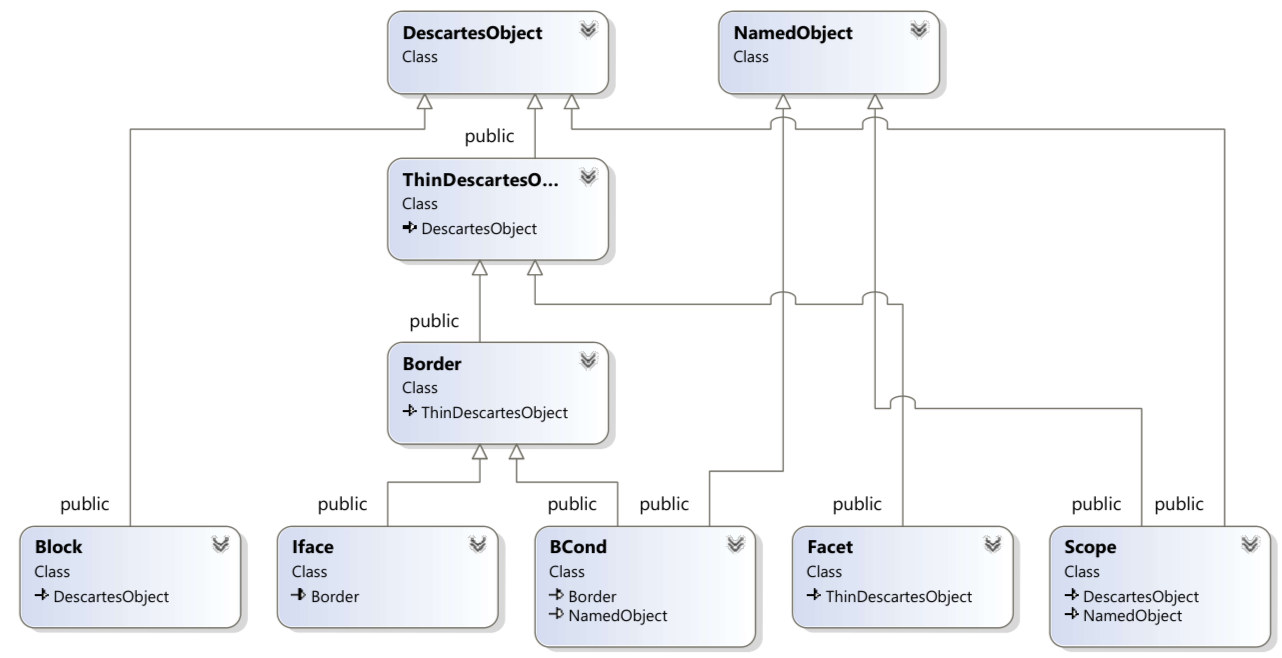
\includegraphics[width=0.8\textwidth]{./pics/text_2_block/9-hierarchy.png}
\singlespacing
\captionstyle{center}\caption{Иерархия объектов внутреннего представления сетки.}
\label{fig:text_2_block_hierarchy}
\end{figure}

\subsubsection{Организация межпроцессных обменов данными между \\ блоками сетки}

Рассмотрим механизм обмена данными между блоками сетки.
Как уже упоминалось, если два соседние блока, между которыми должен быть осуществлен обмен данными, обрабатываются в разных процессах при выполнении расчетов на суперкомпьютере, то обмен данными может быть осуществлен с помощью MPI\label{abbr:mpi2} пересылок.
При этом каждый блок должен отправить своим соседям только данные, находящиеся в его интерфейсных ячейках (могут существовать интерфейсные ячейки, данные из которых требуется отправить сразу двум или трем блокам).
Получить же должен блок те данные, которые соответствуют ячейкам его теневого слоя.

Логика обменов устроена следующим образом.
Так как пара смежных интерфейсов определяет факт касания двух блоков, между которыми должен произойти обмен, то на каждом из этих интерфейсов заводится буфер для данных обмена, после чего происходит обмен данными буферами (см. рис.~\ref{fig:text_2_block_data_exchange}).
Обмены данными происходят одновременно по всем интерфейсам сетки с помощью асинхронных функций
\texttt{MPI\_Isend}, \texttt{MPI\_Irecv}.
Рассмотрим механизм обмена данными между соседними блоками, находящимися в разных процессах, более подробно.

\begin{figure}[ht]
\centering
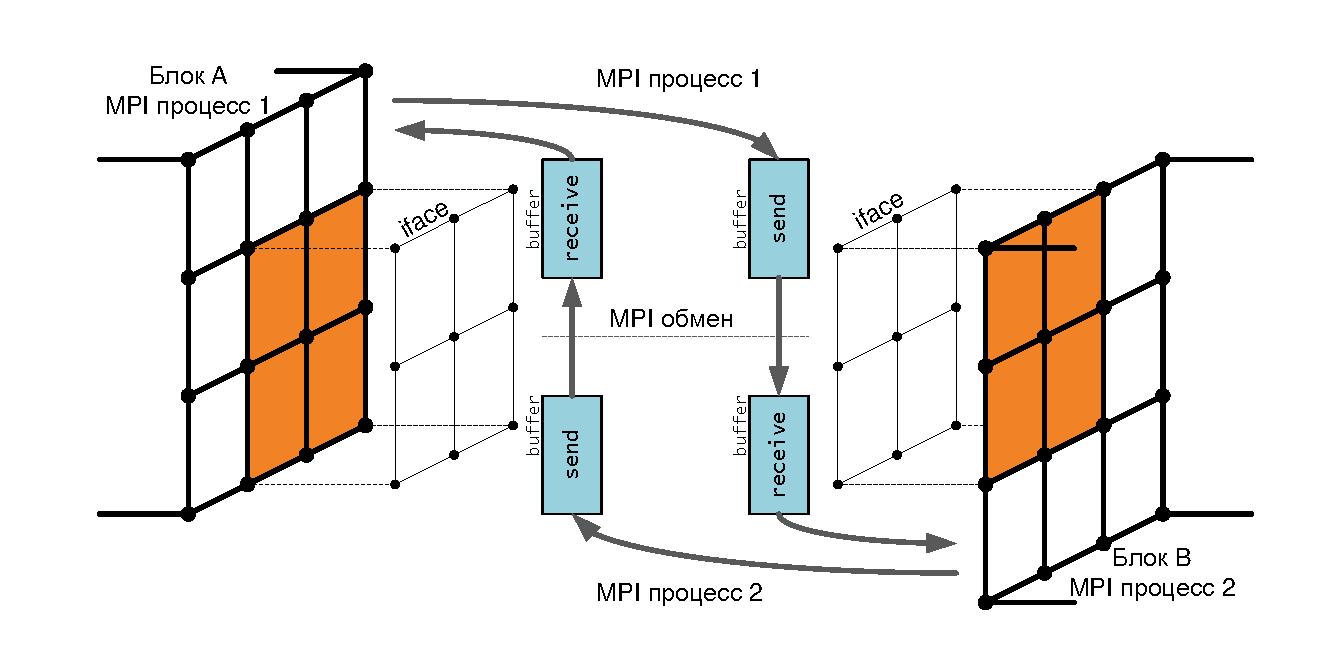
\includegraphics[width=0.8\textwidth]{./pics/text_2_block/10-data-exchange.pdf}
\singlespacing
\captionstyle{center}\caption{Обмен данными между блоками сетки.}
\label{fig:text_2_block_data_exchange}
\end{figure}

Пусть Блок A обрабатывается в процессе 1, а блок B -- в процессе 2, как показано на рис.~\ref{fig:text_2_block_data_exchange}.
Каждый из двух смежных интерфейсов, описывающих касание этих двух блоков имеет свой буфер обмена данными.
Так как в процессе 1 активным является блок A, то буфер его интерфейса работает на прием данных, а буфер интерфейса со стороны блока B -- на отправку (данных блока A).
В процессе 2 все происходит ровно наоборот: активным является блок B, буфер интерфейса блока A работает на отправку данных блока B, буфер интерфейса со стороны блока B работает на прием данных.
Для всех интерфейсов происходит асинхронный запуск всех вызовов функций обмена, после чего происходит ожидание завершения всех операций.
После этого каждый блок может извлечь данный из буфера интерфейса, в котором он является активным, и поместить эти данные в свою теневую зону, после чего начинается следующая итерация расчетов.

\begin{figure}[ht]
\centering
\begin{tabular}{l}
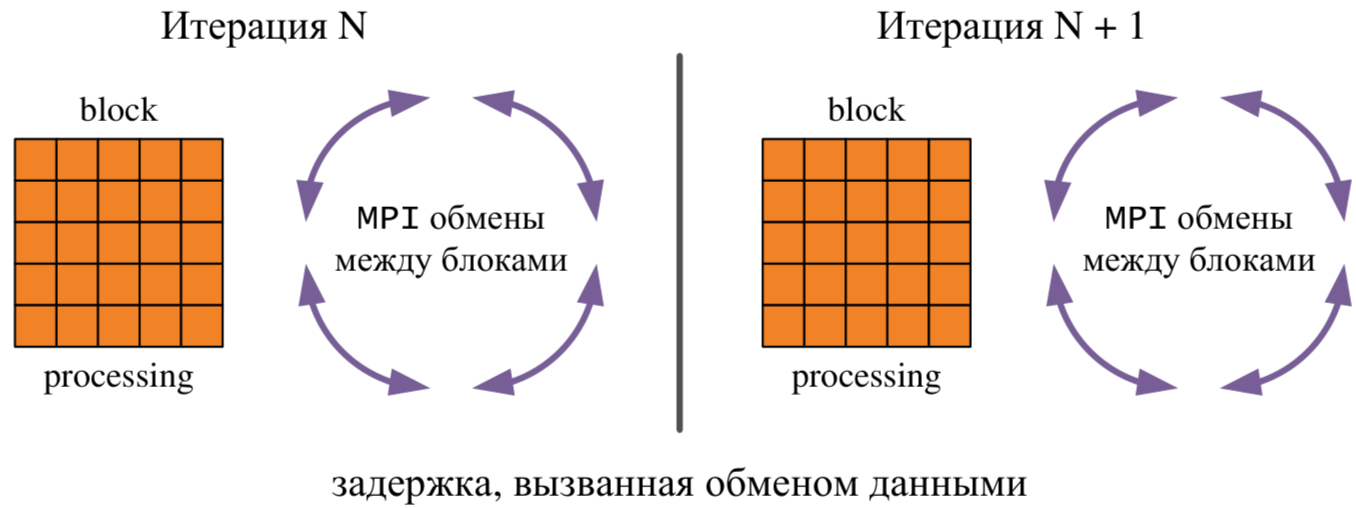
\includegraphics[width=0.6\textwidth]{./pics/text_2_block/11-mpi1.png}
\\
\\
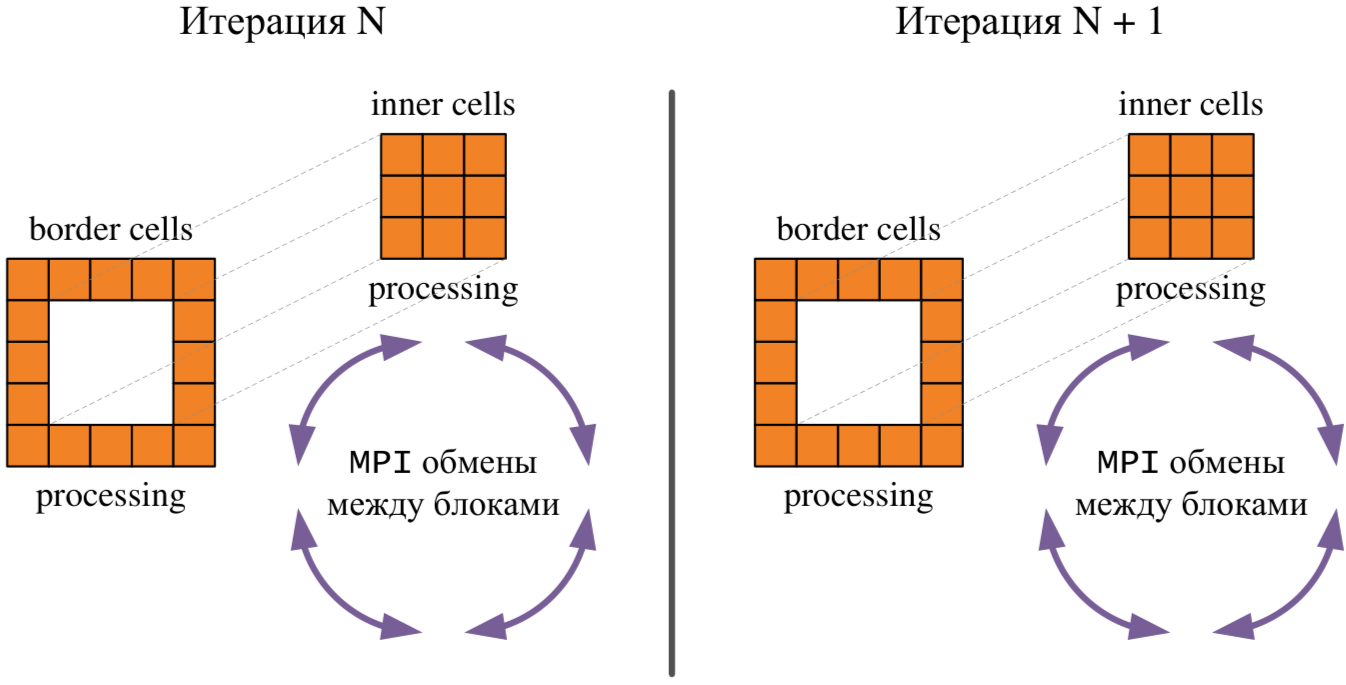
\includegraphics[width=0.6\textwidth]{./pics/text_2_block/12-mpi2.png}
\end{tabular}
\singlespacing
\captionstyle{center}\caption{Задержки, вызванные MPI обменами и избавление от них.}
\label{fig:text_2_block_mpi1}
\end{figure}

После проведения каждой итерации счета задачи необходимо выполнять обмен данными, чтобы состояния граничных ячеек блоков были актуальными.
При этом начинать обсчет следующей итерации нельзя до завершения всех обменов.
Это может привести к возникновению задержек (см. рис.~\ref{fig:text_2_block_mpi1}, сверху).
Чтобы избежать такого рода потери вычислительного времени можно разделить обработку ячеек блока на отдельную обработку всех внутренних ячеек и обработку граничных ячеек.
Сначала нужно произвести обработку всех граничных ячеек блока, затем инициировать асинхронные обмены данными (в которых участвуют только граничные ячейки), а затем сразу начать обработку внутренних ячеек, для которых получение данных фиктивных ячеек не требуется.
Такой подход позволяет скрыть издержки на коммуникацию за полезными вычислениями (см. рис.~\ref{fig:text_2_block_mpi1}, снизу).

Особенности структуры и реализации внутреннего представления блочно-структурированной сетки имеют большое значение для выполнения расчетов на этой сетке.
Правильный выбор объектной модели сетки, способы расположения данных в памяти и другие факторы напрямую влияют на эффективность выполнения программы.
Важную роль в скорости выполнения расчетов играет реализация механизма обмена данными в случае запуска вычисления на суперкомпьютере.
Так как обмен данными должен происходить на каждой итерации вычислений, то это является узким местом для повышения эффективности расчетов.
